\documentclass[tikz,border=6pt]{standalone}
\usepackage{pgfplots}
\pgfplotsset{compat=1.18}
\usepgfplotslibrary{colormaps}
\usetikzlibrary{arrows, arrows.meta, calc}
\usetikzlibrary{decorations.markings}


\usepackage{amssymb,amsmath,mathtools}

\usepackage[T1]{fontenc}
\usepackage[utf8]{inputenc}
\usepackage{newpxtext,newpxmath}
\usepackage{sectsty}

\newcommand{\Arg}{\textrm{Arg}}

\renewcommand{\Re}{\operatorname{\mathrm{Re}}}
\renewcommand{\Im}{\operatorname{\mathrm{Im}}}

\begin{document}
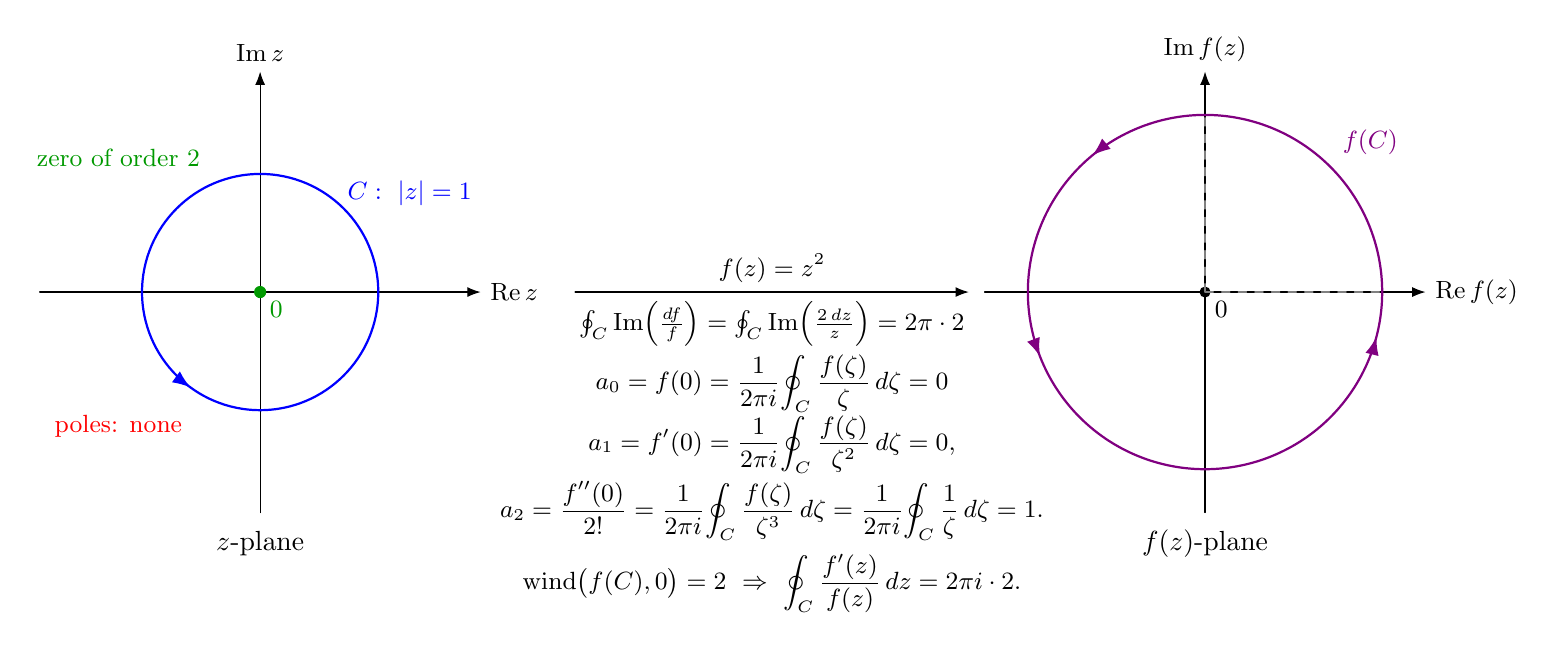
\begin{tikzpicture}[>=Latex, line cap=round, line join=round, font=\small]
%========================
% Left: z-plane
%========================
\begin{scope}[shift={(0,0)}]
	\node[font=\normalsize] at (0,-3.2) {$z$-plane};
	% axes
	\draw[->] (-2.8,0)--(2.8,0) node[right] {$\Re z$};
	\draw[->] (0,-2.8)--(0,2.8) node[above] {$\Im z$};
	
	% unit circle C (positively oriented) -- radius 1.5 for visibility
	\draw[blue,thick,postaction={decorate},
	decoration={markings, mark=at position 0.65 with {\arrow{>}}}]
	(0,0) circle (1.5);
	\node[blue] at (1.9,1.25) {$C:\ |z|=1$};
	
	% zero at 0 (order 2)
	\fill[green!60!black] (0,0) circle(2.2pt) node[below right] {$0$};
	\node[green!60!black] at (-1.8,1.7) {zero of order $2$};
	\node[red] at (-1.8,-1.7) {poles: none};
\end{scope}

% function label + order via winding form
% annotation: Taylor coefficients at z_0=0 via Cauchy integrals
\draw[->] (4,0) -- (9,0) node[midway, above, align=center] {$\displaystyle
	f(z)=z^2$};
\draw[->, opacity=0] (4,0) -- (9,0) node[midway, below, align=center, opacity=1] {
	$\oint_C \operatorname{Im}\!\Big(\frac{df}{f}\Big)
	=\oint_C \operatorname{Im}\!\Big(\frac{2\,dz}{z}\Big)=2\pi\cdot 2$\\[2pt]
	$\displaystyle
	a_0=f(0)=\frac{1}{2\pi i}\!\oint_C \frac{f(\zeta)}{\zeta}\,d\zeta=0$ \\
	$\displaystyle a_1=f'(0)=\frac{1}{2\pi i}\!\oint_C \frac{f(\zeta)}{\zeta^{2}}\,d\zeta=0,$\\[2pt]
	$\displaystyle
	a_2=\frac{f''(0)}{2!}
	=\frac{1}{2\pi i}\!\oint_C \frac{f(\zeta)}{\zeta^{3}}\,d\zeta
	=\frac{1}{2\pi i}\!\oint_C \frac{1}{\zeta}\,d\zeta=1.$\\[4pt]
	$\mathrm{wind}\big(f(C),0\big)=2
	\ \Rightarrow\
	\displaystyle \oint_C \frac{f'(z)}{f(z)}\,dz=2\pi i\cdot 2.$};

%========================
% Right: f(z)-plane
%========================
\begin{scope}[shift={(12,0)}]
	\node[font=\normalsize] at (0,-3.2) {$f(z)$-plane};
	% axes
	\draw[->] (-2.8,0)--(2.8,0) node[right] {$\Re f(z)$};
	\draw[->] (0,-2.8)--(0,2.8) node[above] {$\Im f(z)$};
	
	% origin
	\fill (0,0) circle(2pt) node[below right] {$0$};
	
	% image curve f(C): z = 1.5 e^{it} -> w = (1.5)^2 e^{i 2t}
	\draw[violet,thick,
	postaction={decorate},
	decoration={markings,
			mark=at position 0.18 with {\arrow{>}},
			mark=at position 0.48 with {\arrow{>}},
			mark=at position 0.78 with {\arrow{>}}}]
	plot[domain=0:6.283, samples=520]
	({ (1.5*1.5)*cos(2*\x r) },{ (1.5*1.5)*sin(2*\x r) });
	\node[violet] at (2.1,1.9) {$f(C)$};
	
	% dashed rays to visualize winding
	\draw[gray,dashed] (0,0) -- (2.3,0);
	\draw[gray,dashed] (0,0) -- (0,2.3);
\end{scope}
\end{tikzpicture}
\end{document}